\documentclass[tikz,border=2pt]{standalone}
\usepackage{pgfplots}
\pgfplotsset{compat=1.18}
\usetikzlibrary{intersections}
\usepgfplotslibrary{fillbetween}


\begin{document}
	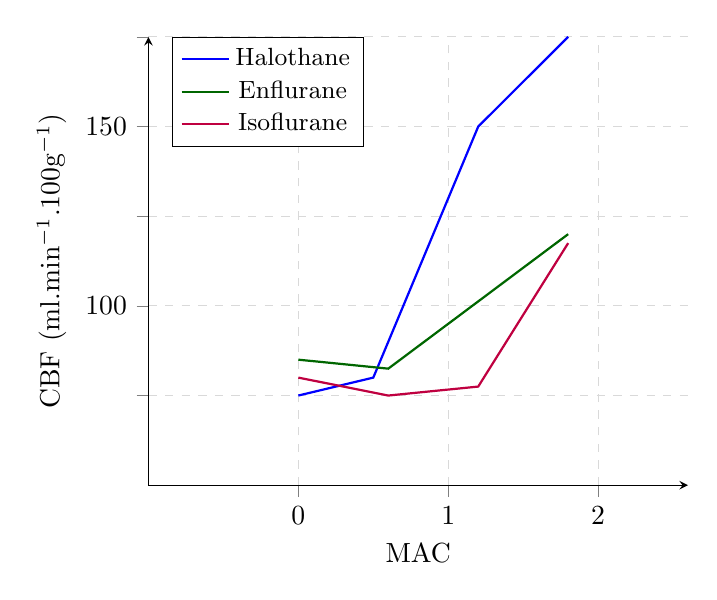
\begin{tikzpicture}
		\begin{axis}[
			axis lines=middle,
			ymin = 0,
			ymax = 5,
			xmin = 0,
			xmax= 1.8,
			grid = major,
			grid style={dashed, gray!30},
			ylabel near ticks,
			xlabel near ticks,
			xlabel= MAC,
			ylabel= CBF (ml.min$^{-1}$.100g$^{-1}$),
			tick align=outside,
			xticklabels={,,0,1,2},
			yticklabels={,,,100,,150},
			legend style={font=\small, cells={align=left},at={(0.4,1)}}]

			\draw [blue, thick] (0.5,1) -- (0.75, 1.2) -- (1.1, 4) -- (1.4, 5);
			\draw [black!60!green, thick] (0.5,1.4) -- (0.8, 1.3) -- (1.4, 2.8);
			\draw [purple, thick] (0.5,1.2) -- (0.8, 1) -- (1.1, 1.1) -- (1.4, 2.7);

			%\draw [black, thick] (0.8,0.5) -- (4.2,1.5);
			%\draw [blue, thick] (0.7,0.75) -- (3.8,2.3);
			%\draw [red, thick] (0.5,0.8) -- (1.8,4.8);


		\addlegendimage{blue, thick};
		\addlegendentry{Halothane};
		\addlegendimage{black!60!green, thick, thick};
		\addlegendentry{Enflurane};
		\addlegendimage{purple, thick};
		\addlegendentry{Isoflurane};


		\end{axis}
	\end{tikzpicture} 
\end{document}